\section{Finite Markov Decision Processes}

\subsection{The Agent-Environment Interface}
\begin{figure}[h!]
	\centering
	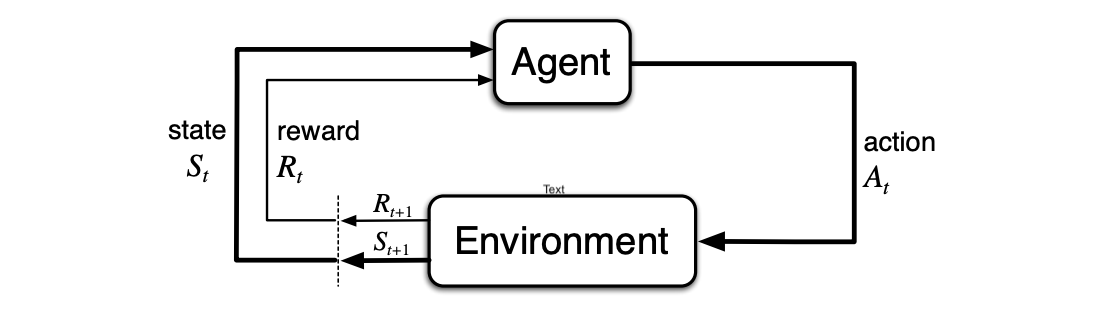
\includegraphics[width=\textwidth]{/chapter3_1}
	\caption{The agent-environment interface in reinforcement learning}
	\label{fig:agent-environment}
\end{figure}

\begin{itemize}
	\item At each timestep the agent implements a mapping from states to probabilities of selecting a possible action. The mapping is called the agents \textit{policy}, denoted \(\pi\), where \(\pi(a | s)\) is the probability of the agent selecting actions a in states.
	\item In general, actions can be any decision we want to learn how to make, and states can be any interpretation of the world that might inform those actions.
	\item The boundary between agent and environment is much closer to the agent than is first intuitive. E.g. if we are controlling a robot, the voltages or stresses in its structure are part of the environment, not the agent. Indeed reward signals are part of the environment, despite very possibly being produced by the agent e.g. dopamine.
\end{itemize}

\subsection{Goals and Rewards}
The \textit{reward hypothesis}:
\begin{displayquote}
	All we mean by goals and purposes can be well thought of as the maximization of the expected value of the cumulative sum of a received scalar signal (called reward).
\end{displayquote}

The reward signal is our way of communicating to the agent what we want to achieve not how we want to achieve it.

\subsection{Returns and Episodes}
The return \(G_t\) is the sum of future rewards:

\begin{equation}
	G_t = R_{t+1} + R_{t+2} + R_{t+3} + \cdots + R_t
\end{equation}

\begin{itemize}
	\item This approach makes sense in applications that finish, or are periodic. That is, the agent-environment interaction breaks into \textit{episodes}.
	\item We call these systems \textit{episodic tasks}. e.g playing a board game, trips through a maze etc.
	\item Notation for state space in an episodic task varies from the conventional case (\(s \in \mathcal{S}\)) to (\(s \in \mathcal{S^+}\))
	\item The opposite, continuous applications are called \textit{continuing tasks}.
	\item For these tasks we use \textit{discounted returns} to avoid a sum of returns going to infinity.
\end{itemize}

\begin{equation}
	G_t = R_{t+1} + \gamma R_{t+2} + \gamma^2 R_{t+3} + \cdots = \sum_{k=0}^{\infty} \gamma^k R_{t+k+1} 
\end{equation}

If the reward is a constant + 1 at each timestep, cumulative discounted reward $G_t$ becomes:

\begin{equation}
G_t = \sum_{k=0}^{\infty} \gamma^k = \frac{1}{1 - \gamma}
\end{equation}

\textit{Discounting} is a crucial topic in RL. It allows us to store a finite value of any state (summarised by its expected cumulative reward) for continuous tasks, where the non-discounted value would run to infinity. 

\subsection{Unified Notation for Episodic and Continuing Tasks}
\begin{equation}
	G_t = \sum_{k=0}^{T-t-1} \gamma^k R_{t+k+1} 
\end{equation}

\subsection{The Markov Property}
A state signal that succeeds in retaining all relevant information about the past is \textit{Markov}. Examples include:
\begin{itemize}
\item A cannonball with known position, velocity and acceleration
\item All positions of chess pieces on a chess board.
\end{itemize}

In normal causal processes, we would think that our expectation of the state and reward at the next timestep is a function of all previous states, rewards and actions, as follows:

\begin{equation}
	Pr \{R_{t+1} = r, S_{t+1} = s' | S_0, A_0, R_1, \ldots, S_{t-1}, A_{t-1}, R_t, S_t, A_t\}  
\end{equation}

If the state is Markov, however, then the state and reward right now completely characterizes the history, and the above can be reduced to:

\begin{equation}
p(s', r | s, a) = Pr \{R_{r+1} = r, S_{t+1} = s' | S_t, A_t\}
\end{equation}

\begin{itemize}
\item Even for non-Markov states, it is appropriate to think of all states as at least an approximation of a Markov state.
\item Markov property is important in RL because decisions and values are assumed to be a function only of the current state.
\item Most real scenarios are unlikely to be Markov. In the example of controlling HVAC, the HVAC motor might heat up which affects cooling power and we may not be tracking that temperature. It is hard for a process to be Markov without sensing all possible variables.
\end{itemize}

\subsection{Markov Decision Process (MDP)}
Given any state and action s and a, the probability of each possible pair of next state and reward, s', r is denoted:

\begin{equation}
p(s', r | s, a) = Pr \{R_{r+1} = r, S_{t+1} = s' | S_t, A_t\}
\end{equation}

We can think of \(p(s', r | s, a)\) as the dynamics of our MDP, often called the \textit{transition function}–it defines how we move from state to state given actions. 

\subsection{Policies and Value Functions}
\begin{itemize}
\item Value functions are functions of states or functions of state-value pairs.
\item They estimate how good it is to be in a given state, or how good it is to perform a given action in a given state.
\item Given future rewards are dependent on future actions, value functions are defined with respect to particular policies as the value of a state depends on the action an agent takes in said state.
\item A \textit{policy} is a mapping from states to probabilities of selecting each possible action.
\item RL methods specify how the agent's policy changes as a result of its experience.
\item For MDPs, we can define nu-pi(s) formally as:
\end{itemize}

\begin{equation}
v_\pi(s) = \mathbb{E}_\pi \left[G_t | S_t = s \right] = \mathbb{E}_\pi \left[\sum_{k=0}^{\infty} \gamma^k R_{t+k+1} | S_t = s\right]
\end{equation}

i.e. the expected future rewards, given state \(S_t\), and policy \(\pi\). We call \(v_\pi(s)\)the \textbf{state value function for policy \(pi\)}. Similarly, we can define the value of taking action \(a\) in state \(s\) under policy \(\pi\) as:

\begin{equation}
q_\pi(s,a) = \mathbb{E}_\pi \left[G_t | S_t = s, A_t = a \right] = \mathbb{E}_\pi \left[\sum_{k=0}^{\infty} \gamma^k R_{t+k+1} | S_t = s, A_t = a \right]
\end{equation}

i.e. the expected value, taking action \(a\) in state \(s\) then following policy \(\pi\).
\begin{itemize}
\item We call \(q_\pi\) the \textbf{action-value function for policy \(\pi\)}
\item Both value functions are estimated from experience.
\end{itemize}

A fundamental property of value functions used throughout reinforcement learning and dynamic programming is that they satisfy recursive relationships similar to that which we have already established for the return. This recursive relationship is characterised by the \textbf{Bellman Equation}:

\begin{equation}
v_\pi(s) = \sum_{a} \pi(a|s) \sum_{s',r} p(s', r | s, a) \left[r + \gamma v_\pi(s')\right]
\end{equation}

This recursion looks from one state through to all possible next states given our policy and the dynamics as suggested by \ref{fig:backup}:
\begin{figure}[h!]
	\centering
	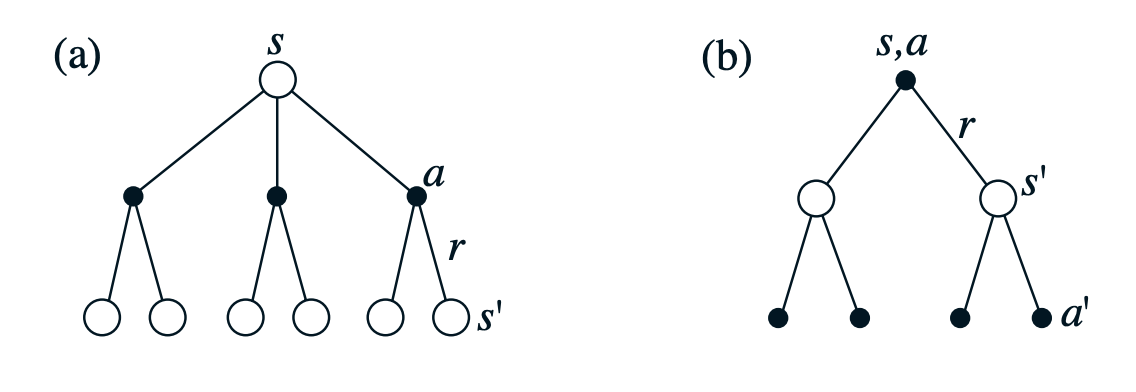
\includegraphics[width=\textwidth]{/chapter3_2}
	\caption{Backup diagrams for \(v_\pi\) and \(q_\pi\)}
	\label{fig:backup}
\end{figure}

\subsection{Optimal Policies and Value Functions}
\begin{itemize}
\item A policy \(\pi '\) is defined as better than policy pi if its expected return is higher for all states.
\item There is always AT LEAST one policy that is better than or equal to all other policies - this is the \textit{optimal policy}.
\item Optimal policies are denoted \(\pi*\)
\item Optimal state-value functions are denoted \(v*\)
\item Optimal action-value functions are denoted \(q*\)
\item We can write \(q*\) in terms of \(v*\):
\end{itemize}

\begin{equation}
q_*(s,a) = \mathbb{E} \left[R_{t+1} + \gamma v_*(S_{t+1}) | S_t = s, A_t = a \right]
\end{equation}

We can adapt the Bellman equation to achieve the Bellman optimality equation, which takes two forms. Firstly for \(v_*\):
\begin{equation}
v_*(s) = \max_{a \in \mathcal{A}(s)} \sum_{s',r} p(s', r | s, a) \left[r + \gamma v_*(s')\right]
\end{equation}
and secondly for \(q_*\):
\begin{equation}
q_*(s) = \sum_{s',r} p(s', r | s, a) \left[r + \gamma \max_{a'} q_*(s', a') \right]
\end{equation}

\begin{itemize}
\item Using \(v*\) the optimal expected long term return is turned into a quantity that is immediately available for each state. Hence a one-step-ahead search, acting greedily, yield the optimal long-term actions.
\item Fully solving the Bellman optimality equations can be hugely expensive, especially if the number of states is huge, as is the case with most interesting problems.
\item Solving the Bellman optimality equation is akin to exhaustive search. We play out \textit{every} possible scenario until the terminal state and collect their expected reward. Our policy then defines the action that maximises this expected reward. 
\item In the continuous case the Bellman optimality equation is unsolvable as the recursion on the next state's value function would never end.
\end{itemize}

\subsection{Optimality and Approximation}
\begin{itemize}
	\item We must approximate because calculation of optimality is too expensive.
	\item A nice way of doing this is allowing the agent to make sub-optimal decisions in scenarios it has low probability of encountering. This is a trade off for being optimal in situations that occur frequently.
\end{itemize}

\subsection{Key Takeaways}
\begin{itemize}
\item We summarise our goal for the agent as a \textit{reward}; its objective is to maximise the cumulative sum of future rewards
\item For episodic tasks, returns terminate (and are backpropogated) when the episode ends. For the continuous control case, returns are discounted so they do not run to infinity. 
\item A state signal that succeeds in retaining all relevant information about the past is \textit{Markov}. 
\item Markov Decision Processes (MDPs) are the mathematically idealised version of the RL problem. They have system dynamics: $p(s', r | s, a) = Pr \{R_{r+1} = r, S_{t+1} = s' | S_t, A_t\}$
\item Policies are a (probabilistic) mapping from states to actions.
\item Value functions estimate how good it is for an agent to be in a state ($v_\pi$) or to take an action from a state ($q_\pi$). They are always defined w.r.t policies as the value of a state depends on the policy one takes in that state. Value functions are the e\textit{expected cumulative sum of future rewards} from a state or state-action pair.
\item Knowing our policy and system dynamics, we can define the state value function is defined by the Bellman equation: $v_\pi(s) = \sum_{a} \pi(a|s) \sum_{s',r} p(s', r | s, a) \left[r + \gamma v_\pi(s')\right]$
\item An optimal policy ($\pi_*$) is the policy that maximises expected cumulative reward from all states. From the optimal policy we can derive the optimal value functions $q_*$ and $v_*$.
\end{itemize}










